\documentclass{standalone}

\usepackage{fontspec}
\setmainfont{osifont.ttf}
\fontsize{3.5mm}{4mm}\selectfont

\usepackage{tikz}

\newcommand\pageheight{420mm}
\newcommand\pagewidth{594mm}

\newcommand\contentleft{20mm}
\newcommand\contenttop{10mm}
\newcommand\contentright{\pagewidth-10mm}
\newcommand\contentbottom{\pageheight-10mm}

\newcommand\gridsize{5mm}

\newcommand\formatname{A2}

\begin{document}
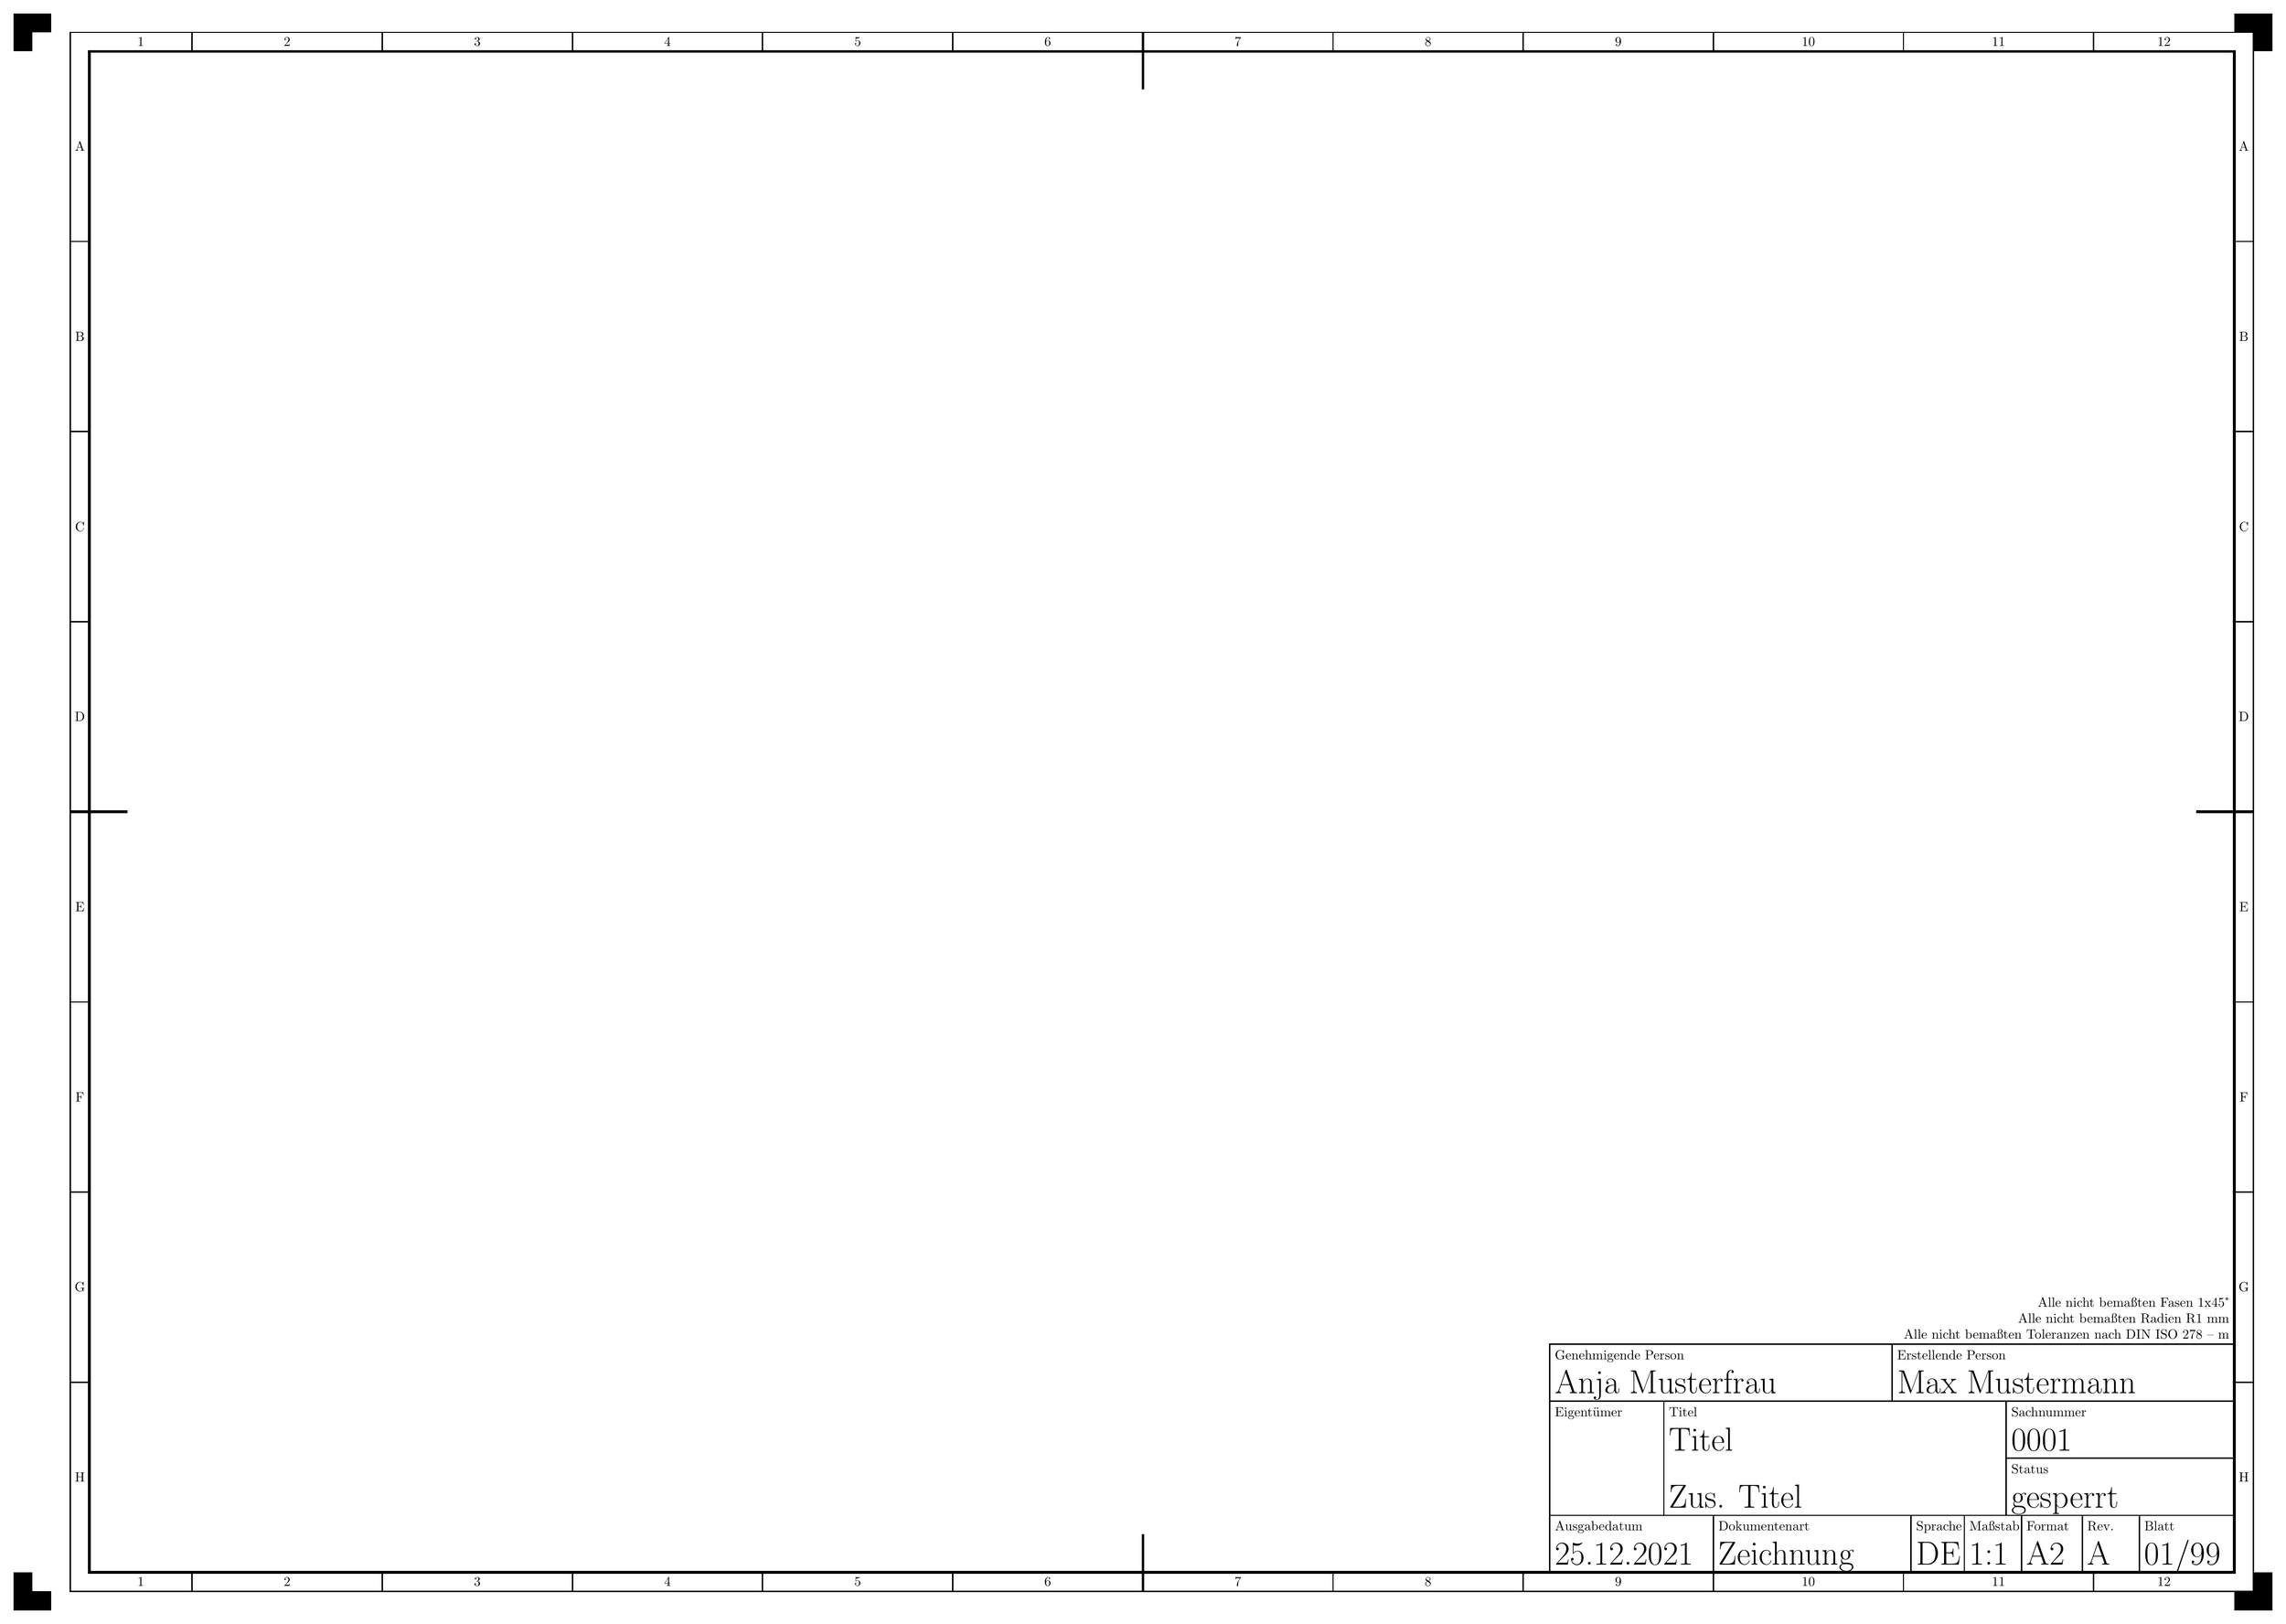
\begin{tikzpicture}[yscale = -1, line width = 0.35mm]
	\fill (0, 0) rectangle +(10mm, 5mm);
	\fill (0, 0) rectangle +(5mm, 10mm);
	\fill (\pagewidth, 0) rectangle +(-5mm, 10mm);
	\fill (\pagewidth, 0) rectangle +(-10mm, 5mm);
	\fill (0, \pageheight) rectangle +(5mm, -10mm);
	\fill (0, \pageheight) rectangle +(10mm, -5mm);
	\fill (\pagewidth, \pageheight) rectangle +(-5mm, -10mm);
	\fill (\pagewidth, \pageheight) rectangle +(-10mm, -5mm);

	% Zeichenbereich:
	\draw [line width = 0.7mm] (\contentleft, \contenttop) rectangle (\contentright, \contentbottom);

	% Mittellinien:
	\begin{scope}[line width = 0.7mm, line join = round]
		\draw (\contentleft-\gridsize, \pageheight/2) -- (\contentleft+10mm, \pageheight/2);
		\draw (\contentright+\gridsize, \pageheight/2) -- (\contentright-10mm, \pageheight/2);
		\draw (\pagewidth/2, \contenttop-\gridsize) -- (\pagewidth/2, \contenttop+10mm);
		\draw (\pagewidth/2, \contentbottom+\gridsize) -- (\pagewidth/2, \contentbottom-10mm);
	\end{scope}

	% Feldeinteilung, muss manuell eingestellt werden
	\draw (\contentleft-\gridsize, \contenttop-\gridsize) rectangle (\contentright+\gridsize, \contentbottom+\gridsize);
	\foreach \y in {60mm, 110mm, 160mm, 260mm, 310mm, 360mm} {
		\draw (\contentleft, \y) -- +(-\gridsize, 0);
		\draw (\contentright, \y) -- +(\gridsize, 0);
	}
	\foreach \y/\label in {35mm/A, 85mm/B, 135mm/C, 185mm/D, 235mm/E, 285mm/F, 335mm/G, 385mm/H} {
		\node at (\contentleft - \gridsize/2, \y) {\label};
		\node at (\contentright + \gridsize/2, \y) {\label};
	}
	
	\foreach \x in {47mm, 97mm, 147mm, 197mm, 247mm, 347mm, 397mm, 447mm, 497mm, 547mm} {
		\draw (\x, \contenttop) -- +(0, -\gridsize);
		\draw (\x, \contentbottom) -- +(0, \gridsize);
	}
	\foreach \x/\label in {
		33.5mm/1, 72mm/2, 122mm/3, 172mm/4, 222mm/5, 272mm/6, 322mm/7, 372mm/8, 422mm/9, 472mm/10, 
		522mm/11, 565.5mm/12
	} {
		\node at (\x, \contenttop - \gridsize/2) {\label};
		\node at (\x, \contentbottom + \gridsize/2) {\label};
	}

	% Schriftfeld
	\draw (\contentright, \contentbottom) rectangle (\contentright-180mm, \contentbottom-60mm);
	\begin{scope}[anchor = base west, xshift = \contentright-180mm, yshift = \contentbottom-60mm]
		% Zeilen
\draw (0mm, 15mm) -- (180mm, 15mm);
\draw (0mm, 45mm) -- (180mm, 45mm);

% Zeile 1
\node at (0mm, 4mm) {Genehmigende Person};
\node at (0mm, 13mm) {\fontsize{10mm}{11mm}\selectfont Anja Musterfrau};
\node at (90mm, 4mm) {Erstellende Person};
\node at (90mm, 13mm) {\fontsize{10mm}{11mm}\selectfont Max Mustermann};
\foreach \x in {90mm} {
	\draw (\x, 0mm) -- (\x, 15mm);
}

% Zeile 2
\node at (0mm, 19mm) {Eigentümer};
\node at (30mm, 19mm) {Titel};
\node at (30mm, 28mm) {\fontsize{10mm}{11mm}\selectfont Titel};
\node at (30mm, 43mm) {\fontsize{10mm}{11mm}\selectfont Zus. Titel};
\foreach \x in {30mm, 120mm} {
	\draw (\x, 15mm) -- (\x, 45mm);
}
\draw (120mm, 30mm) -- (180mm, 30mm);
\node at (120mm, 19mm) {Sachnummer};
\node at (120mm, 28mm) {\fontsize{10mm}{11mm}\selectfont 0001};
\node at (120mm, 34mm) {Status};
\node at (120mm, 43mm) {\fontsize{10mm}{11mm}\selectfont gesperrt};

% Zeile 3
\node at (0mm, 49mm) {Ausgabedatum};
\node at (0mm, 58mm) {\fontsize{10mm}{11mm}\selectfont 25.12.2021};
\node at (43mm, 49mm) {Dokumentenart};
\node at (43mm, 58mm) {\fontsize{10mm}{11mm}\selectfont Zeichnung};
\node at (95mm, 49mm) {Sprache};
\node at (95mm, 58mm) {\fontsize{10mm}{11mm}\selectfont DE};
\node at (109mm, 49mm) {Maßstab};
\node at (109mm, 58mm) {\fontsize{10mm}{11mm}\selectfont 1:1};
\node at (124mm, 49mm) {Format};
\node at (124mm, 58mm) {\fontsize{10mm}{11mm}\selectfont \formatname};
\node at (140mm, 49mm) {Rev.};
\node at (140mm, 58mm) {\fontsize{10mm}{11mm}\selectfont A};
\node at (155mm, 49mm) {Blatt};
\node at (155mm, 58mm) {\fontsize{10mm}{11mm}\selectfont 01/99};
\foreach \x in {43mm, 95mm, 109mm, 124mm, 140mm, 155mm} {
	\draw (\x, 45mm) -- (\x, 60mm);
}

	\end{scope}

	% Weitere Hinweise
	\begin{scope}[anchor = south east]
		\node [align = right] at (\contentright, \contentbottom-60mm) {Alle nicht bemaßten Fasen 1x45°\\Alle nicht bemaßten Radien R1 mm\\Alle nicht bemaßten Toleranzen nach DIN ISO 278 -- m};
	\end{scope}
\end{tikzpicture}
\end{document}
